% ===============================================================
%  جلسه بیستم
% ===============================================================
\chapter{تخمین میانگین مربع و مقدمه تخمین نقطه‌ای}

\section{تخمین میانگین مربع \lr{(Mean Square Estimation)}}

\subsection{تخمین‌گر میانگین مربع}
\begin{itemize}
\item در این نوع از تخمین‌گرها، بر خلاف سناریوهای آماری مطرح شده در جلسات قبل، تعدادی نمونه از متغیر(های) تصادفی موجود نبوده و به جای آن \textbf{خود توزیع مشترک} را در اختیار داریم.
\item \textcolor{red!70!black}{\textbf{حالت ساده:}} هدف، یافتن یک تابع بهینه برای تخمین زدن مقدار متغیر تصادفی $Y$ به فرض دانستن مقدار متغیر تصادفی $X$ است، به شرط آنکه توزیع مشترک $f_{XY}(x,y)$ در دسترس باشد.
\item \textcolor{red!70!black}{\textbf{حالت پیچیده:}} هدف می‌تواند تخمین بهینه چند متغیر تصادفی از روی چند متغیر تصادفی دیگر باشد.
\item این شکل از تخمین (تحت شرایطی) در مبحث \textbf{پیش‌بینی} نیز کاربرد فراوان دارد (مثلاً پیش‌بینی قیمت فردا از روی قیمت امروز، یا تخمین سیگنال ارسالی از روی سیگنال نویزی دریافتی).
\end{itemize}
معیار بهینگی در همه این بخش‌ها \textbf{خطای میانگین مربعات} (\lr{Mean Squared Error, MSE}) است.

\subsection{تخمین غیرشرطی \lr{(Unconditional)}}
\begin{question}[{متغیر تصادفی $X$ با چگالی معلوم $f_X(x)$ را در نظر بگیرید. می‌خواهیم آن را با مقدار ثابت $c$ تخمین بزنیم؛ $c$ را چنان بیابید که $\mathrm{MSE}=\E[(X-c)^2]$ کمینه شود.}]
\begin{answer}
عبارت
\[
\E\big[(X-c)^2\big]=\int_\R(x-c)^2f_X(x)\dd x
\]
به صورت تابعی از مقدار نامعلوم $c$ قابل نوشتن است. از طرفی واضح است که در حدود $c\to\pm\infty$ مقدار خطای میانگین مربع به سمت بی‌نهایت میل می‌کند. در نتیجه، تابع فوق به ازای مقداری از $c$ کمینه است. این مقدار را با استفاده از مشتق‌گیری پیدا می‌کنیم:
\[
\frac{\partial}{\partial c}\E\big[(X-c)^2\big]=\E\big[2(c-X)\big]=0\ \Rightarrow\ \boxed{\ c=\E(X)\ }
\]
کمینه خطا برابر $\E[(X-\E X)^2]=\Var(X)$ است. (معادلاً: $\E(X-c)^2=\Var X+(\E X-c)^2$.)
\end{answer}
\end{question}

\subsection{تخمین‌گر \lr{MS} خطی همگن}
\begin{question}[{متغیرهای $X,Y$ با چگالی مشترک معلوم $f_{XY}$ را در نظر بگیرید. می‌خواهیم $Y$ را به شکل $\hat Y=aX$ از روی $X$ تخمین بزنیم. ضریب $a$ را چنان بیابید که $\E[(Y-aX)^2]$ کمینه شود.}]
\begin{answer}
مشابه با قبل عمل می‌کنیم:
\[
\E\big[(Y-aX)^2\big]=\iint_{\R^2}(y-ax)^2f_{XY}(x,y)\dd x\dd y .
\]
بعد از مشتق‌گیری خواهیم داشت:
\[
\frac{\partial}{\partial a}\E\big[(Y-aX)^2\big]=\E\big[2X(aX-Y)\big]=0\ \Rightarrow\ \boxed{\ a=\frac{\E(XY)}{\E(X^2)}=\frac{m_{1,1}}{m_{2,0}}\ }
\]
\end{answer}
\end{question}

\subsection{تخمین‌گر \lr{MS} خطی غیرهمگن}
\begin{question}[{این بار $Y$ را به شکل $\hat Y=aX+b$ تخمین می‌زنیم. ضرایب $a,b$ را چنان بیابید که $\E[(Y-aX-b)^2]$ کمینه شود.}]
\begin{answer}
مشابه با قبل عمل می‌کنیم، اما این بار دو مجهول داریم:
\[
\E\big[(Y-aX-b)^2\big]=\iint_{\R^2}(y-ax-b)^2f_{XY}(x,y)\dd x\dd y .
\]
بعد از مشتق‌گیری خواهیم داشت:
\[
\frac{\partial}{\partial a}\E\big[(Y-aX-b)^2\big]=\E\big[2X(aX+b-Y)\big]=0\ \Rightarrow\ a\E(X^2)+b\E(X)=\E(XY),
\]
\[
\frac{\partial}{\partial b}\E\big[(Y-aX-b)^2\big]=\E\big[2(aX+b-Y)\big]=0\ \Rightarrow\ b=\E(Y)-a\E(X).
\]
با جایگذاری $b$ در معادله اول: $a\big(\E X^2-(\E X)^2\big)=\E(XY)-\E X\E Y$؛ پس
\[
\boxed{\ a=\frac{\E(XY)-\E(X)\E(Y)}{\E(X^2)-\E^2(X)}=\frac{\sigma_{XY}}{\sigma_X^2}\quad,\quad b=\mu_Y-\frac{\sigma_{XY}}{\sigma_X^2}\mu_X\ }
\]
که در آن $\sigma_{XY}=\Cov(X,Y)$.
\end{answer}
\end{question}

\begin{theorem}[خطای تخمین‌گر خطی بهینه]
با $\hat Y=\mu_Y+\frac{\sigma_{XY}}{\sigma_X^2}(X-\mu_X)$:
\[
\mathrm{MSE}_{\min}=\E\big[(Y-\hat Y)^2\big]=\sigma_Y^2(1-\rho_{XY}^2),
\]
و خطای تخمین $e=Y-\hat Y$ با $X$ ناهمبسته است: $\E[eX]=0$ و $\E[e]=0$ (\textbf{اصل تعامد}).
\end{theorem}
\begin{proof}
$Y-\hat Y=(Y-\mu_Y)-a(X-\mu_X)$ با $a=\sigma_{XY}/\sigma_X^2$. پس
$\E(Y-\hat Y)^2=\sigma_Y^2-2a\sigma_{XY}+a^2\sigma_X^2=\sigma_Y^2-\frac{\sigma_{XY}^2}{\sigma_X^2}=\sigma_Y^2\big(1-\frac{\sigma_{XY}^2}{\sigma_X^2\sigma_Y^2}\big)=\sigma_Y^2(1-\rho^2)$.
اصل تعامد همان دو معادله مشتق برابر صفر است.
\end{proof}
\begin{note}
\notetitle این نتیجه تعبیر عملیاتی زیبایی به ضریب همبستگی می‌دهد: $\rho^2$ کسری از واریانس $Y$ است که به کمک یک تابع خطی از $X$ «توضیح داده می‌شود». اگر $\rho=0$ آنگاه $a=0$ و بهترین تخمین خطی همان ثابت $\mu_Y$ است ($X$ هیچ کمکی نمی‌کند). اگر $|\rho|=1$ خطا صفر است. \textbf{تعبیر هندسی:} اگر متغیرهای تصادفی با میانگین صفر را بردار و $\E[UV]$ را ضرب داخلی بگیریم، $\hat Y$ تصویر عمود $Y$ روی فضای تولیدشده توسط $\{1,X\}$ است و خطا بر این فضا عمود است.
\end{note}

\subsection{تخمین‌گر \lr{MS} غیرخطی}
\begin{question}[{این بار $Y$ را به شکل کلی $\hat Y=\phi(X)$ از روی $X$ تخمین می‌زنیم که تابع دلخواه $\phi(\cdot)$ مجهول است. $\phi$ را چنان بیابید که $\E[(Y-\phi(X))^2]$ کمینه شود.}]
\begin{answer}
این مورد کمی پیچیده‌تر است:
\[
\E\big[(Y-\phi(X))^2\big]=\iint_{\R^2}\big(y-\phi(x)\big)^2f_{XY}(x,y)\dd x\dd y .
\]
از قانون میانگین کل (جلسه چهاردهم) استفاده می‌کنیم:
\[
\E\big[(Y-\phi(X))^2\big]=\E\Big\{\E\big[(Y-\phi(X))^2\,\big|\,X\big]\Big\}=\int\underbrace{\Big(\int\big(y-\phi(x)\big)^2f_{Y|X}(y\given x)\dd y\Big)}_{\text{برای هر $x$ جداگانه}}f_X(x)\dd x .
\]
میانگین داخلی همواره مقداری نامنفی دارد، و برای هر $x$ ثابت، $\phi(x)$ صرفاً یک عدد ثابت است. از بخش «تخمین غیرشرطی» می‌دانیم که کمینه $\E[(Y-c)^2\given X=x]$ در $c=\E(Y\given X=x)$ اتفاق می‌افتد. چون می‌توان برای هر $x$ جداگانه بهترین عدد را انتخاب کرد، کل انتگرال کمینه می‌شود. لذا داریم:
\[
\boxed{\ \phi(X)=\E(Y\given X)\ }
\]
\end{answer}
\end{question}

\begin{summarybox}[نکته مهم]
همواره داریم (روابط زیر از چپ به راست خوانده شوند):
\[
\underbrace{\min_{\phi}\E\big[(Y-\phi(X))^2\big]}_{\text{غیرخطی}}\ \le\ \underbrace{\min_{a,b}\E\big[(Y-aX-b)^2\big]}_{\text{خطی غیرهمگن}}\ \le\ \underbrace{\min_{a}\E\big[(Y-aX)^2\big]}_{\text{خطی همگن}}
\]
و همچنین خطای خطی غیرهمگن از خطای بهترین ثابت ($\sigma_Y^2$) بیشتر نیست. به بیان دیگر: \textbf{خطای \lr{MS} غیرخطی، کمتر یا مساوی خطای \lr{MS} خطی است.}
\end{summarybox}
\begin{question}[چرا؟]
\begin{answer}
زیرا هر تخمین‌گر خطی همگن ($aX$) حالت خاصی از خطی غیرهمگن ($aX+b$ با $b=0$) است، و هر تخمین‌گر خطی، حالت خاصی از تابع کلی $\phi(X)$ است. کمینه گرفتن روی یک مجموعه بزرگ‌تر از توابع، هرگز جواب بدتری نمی‌دهد. به همین ترتیب تخمین ثابت $c=\mu_Y$ (با خطای $\sigma_Y^2$) حالت خاص $a=0$ است.
\end{answer}
\end{question}

\begin{example}[وقتی تخمین‌گر خطی کاملاً شکست می‌خورد]
$X\sim\mathcal U(-1,1)$ و $Y=X^2$. بهترین تخمین‌گرهای خطی و غیرخطی $Y$ از روی $X$ را بیابید.
\begin{solution}
از جلسه پانزدهم، $\Cov(X,Y)=0$؛ پس $a=0$ و $b=\mu_Y=\E X^2=\frac13$. تخمین‌گر خطی: $\hat Y=\frac13$ با خطای $\Var(Y)=\E X^4-\frac19=\frac15-\frac19=\frac{4}{45}$. تخمین‌گر غیرخطی: $\E(Y\given X)=X^2$ که خطای آن \textbf{صفر} است! همبستگی صفر به معنای بی‌اطلاعی نیست؛ فقط یعنی رابطه خطی وجود ندارد.
\end{solution}
\end{example}

\begin{example}[یک مثال عددی]
برای چگالی $f_{XY}=x+y$ روی مربع واحد (جلسه سیزدهم)، تخمین‌گرهای \lr{MS} را بیابید.
\begin{solution}
از جلسه پانزدهم: $\mu_X=\mu_Y=\frac7{12}$، $\sigma_X^2=\sigma_Y^2=\frac{11}{144}$، $\sigma_{XY}=-\frac1{144}$.
\begin{itemize}
\item \textbf{ثابت:} $\hat Y=\frac7{12}$، خطا $\frac{11}{144}\approx0.07639$.
\item \textbf{خطی غیرهمگن:} $a=\frac{-1/144}{11/144}=-\frac1{11}$ و $b=\frac7{12}+\frac1{11}\cdot\frac7{12}=\frac7{11}$؛ پس $\hat Y=\frac{7-X}{11}$، خطا $\frac{11}{144}(1-\frac1{121})\approx0.07576$.
\item \textbf{غیرخطی:} $\E(Y\given X=x)=\frac{\int_0^1y(x+y)\dd y}{x+\frac12}=\frac{x/2+1/3}{x+1/2}$، خطا (محاسبه عددی) $\approx0.07570$.
\end{itemize}
ترتیب خطاها مطابق نکته بالاست. در این مثال وابستگی ضعیف است و بهبودها کوچک‌اند.
\end{solution}
\end{example}

\subsection{توزیع‌های مشترکاً گاوسی}
فرض کنید که متغیرهای تصادفی $X,Y$ مشترکاً گاوسی با میانگین‌های $\mu_X,\mu_Y$، واریانس‌های $\sigma_X^2,\sigma_Y^2$ و ضریب همبستگی $r$ باشند ($\sigma_{XY}=r\sigma_X\sigma_Y$).
\begin{itemize}
\item \textbf{تخمین‌گر \lr{MS} خطی غیرهمگن:}
\[
\hat Y=\frac{r\sigma_X\sigma_Y}{\sigma_X^2}x+\mu_Y-\frac{r\sigma_X\sigma_Y}{\sigma_X^2}\mu_X=\frac{r\sigma_Y}{\sigma_X}(x-\mu_X)+\mu_Y .
\]
\item \textbf{تخمین‌گر \lr{MS} غیرخطی:} از جلسه چهاردهم (توزیع شرطی گاوسی):
\[
\hat Y=\E(Y\given X)=\frac{r\sigma_Y}{\sigma_X}(x-\mu_X)+\mu_Y .
\]
\end{itemize}
توزیع‌های مشترکاً گاوسی از جمله توزیع‌هایی هستند که تخمین‌گرهای خطی غیرهمگن و غیرخطی از حیث خطای \lr{MS} برابرند (تخمین‌گرها یکی هستند). این یکی از دلایل محبوبیت بسیار زیاد مدل‌های گاوسی و فیلترهای خطی (مانند فیلتر وینر و فیلتر کالمن) در مهندسی است.

\subsection{تخمین‌گر \lr{MS} خطی غیرهمگن (چندمتغیره)}
\begin{question}[{متغیرهای تصادفی $X_1,\ldots,X_n,Y$ با چگالی مشترک معلوم را در نظر بگیرید. می‌خواهیم $Y$ را به شکل $\hat Y=a_1X_1+\cdots+a_nX_n+b$ تخمین بزنیم به طوری که $\E[(Y-a_1X_1-\cdots-a_nX_n-b)^2]$ کمینه شود. ضرایب را بیابید.}]
\begin{answer}
مشابه با حالت دو متغیره، با مشتق‌گیری نسبت به هر $a_i$ و $b$، یک دستگاه معادلات $(n+1)$تایی تشکیل می‌دهیم:
\[
\sum_{j=1}^{n}a_j\E(X_iX_j)=\E(X_iY)-b\E(X_i),\qquad i=1,2,\ldots,n,
\]
\[
b=\E(Y)-\sum_{i=1}^{n}a_i\E(X_i).
\]
می‌توان به راحتی دید که دستگاه معادلات بالا خطی بوده و جواب آن از طریق محاسبه یک ماتریس معکوس به دست خواهد آمد. با جایگذاری $b$ در معادلات اول (و نماد برداری $\underline X=(X_1,\ldots,X_n)^T$):
\[
\sum_ja_j\Cov(X_i,X_j)=\Cov(X_i,Y)\quad\Longleftrightarrow\quad\Sigma\,\underline a=\E\big[(\underline X-\E\underline X)(Y-\E Y)\big],
\]
\[
\boxed{\ \underline a=\Sigma^{-1}\E\big[(\underline X-\E\underline X)(Y-\E Y)\big]\quad,\quad b=\E(Y)-\E(\underline X)^T\Sigma^{-1}\big(\E(\underline XY)-\E\underline X\,\E Y\big)\ }
\]
که در اینجا $\Sigma$ ماتریس کوواریانس میان $X$ها است: $\Sigma_{ij}=\Cov(X_i,X_j)$. (برای $n=1$ دقیقاً به $a=\sigma_{XY}/\sigma_X^2$ می‌رسیم.)
\end{answer}
\end{question}

\begin{note}
\notetitle این همان «رگرسیون خطی» در یادگیری ماشین است: وقتی به جای توزیع، نمونه داریم، امیدهای ریاضی را با میانگین‌های تجربی جایگزین می‌کنیم و به روش «کمترین مربعات» ($\hat{\underline a}=(\mathbf X^T\mathbf X)^{-1}\mathbf X^T\mathbf y$) می‌رسیم.
\end{note}

\section{تخمین نقطه‌ای \lr{(Point Estimation)}}

\subsection{مفهوم}
\begin{itemize}
\item تخمین نقطه‌ای، به تخمین پارامتر (یا پارامترهای) یک توزیع آماری از روی مشاهدات به دست آمده از آن اطلاق می‌گردد.
\item به طور دقیق‌تر، فرض کنید متغیر تصادفی $X\sim f_X(x;\theta)$ از توزیعی با پارامتر(های) نامعلوم $\theta$ حاصل شده باشد. فرض کنید $X_1,X_2,\ldots,X_n$ تعدادی نمونه مشاهده شده (یا \lr{realized}) از $X$ باشند. نمونه‌ها می‌توانند \lr{i.i.d.} یا غیر \lr{i.i.d.} باشند.
\item هدف یافتن تابعی مانند $\hat\theta$ است که مشاهدات را به عضوی از فضای پارامترهای $\Theta$ نگاشت دهد.
\item عبارت «تخمین نقطه‌ای» از آن جهت استفاده می‌شود که به دنبال یافتن نقطه‌ای در فضای پارامترها هستیم (در مقابل تخمین بازه‌ای).
\end{itemize}

\begin{warning}
\warntitle دقت کنید که تخمین‌گر $\hat\theta(X_{1:n})$ خود یک \textbf{متغیر تصادفی} بوده و دارای یک توزیع آماری است. ($\theta$ یک عدد ثابت ولی نامعلوم است؛ $\hat\theta$ تابعی از نمونه‌های تصادفی است.)
\end{warning}

\subsection{گرایش \lr{(Bias)}، واریانس \lr{(Variance)} و سازگاری \lr{(Consistency)}}
فرض کنید که توزیع $X\sim f_X(x;\theta)$ توسط فضای پارامتر(های) $\Theta$ پارامتریزه شده باشد. پارامتر(های) $\theta\in\Theta$ توزیع برای ما نامعلوم است. همچنین فرض کنید نمونه‌های $X_1,\ldots,X_n$ \lr{i.i.d.} گرفته شده از این توزیع باشند. تخمین‌گر $\hat\theta=\hat\theta(X_{1:n})$ را در نظر بگیرید:

\begin{definition}[گرایش، واریانس و سازگاری]
\begin{itemize}
\item \textbf{گرایش \lr{(Bias)}:}
$\ \mathrm{Bias}(\hat\theta,\theta)=\E_{X_{1:n}|\theta}\big\{\theta-\hat\theta(X_{1:n})\big\}$.
\item \textbf{واریانس \lr{(Variance)}:}
$\ \Var(\hat\theta,\theta)=\E_{X_{1:n}|\theta}\big\{(\hat\theta-\E\hat\theta)^2\big\}$.
\item تخمین‌گر $\hat\theta$ را \textbf{سازگار} (\lr{Consistent}) می‌نامیم اگر $\ \lim_{n\to\infty}\hat\theta(X_{1:n})=\theta\ $ (در احتمال، یعنی برای هر $\varepsilon>0$: $\Prob(|\hat\theta-\theta|>\varepsilon)\to0$).
\end{itemize}
تخمین‌گری با گرایش صفر را \textbf{بی‌گرایش} (\lr{Unbiased}) می‌نامیم.
\end{definition}
(در بسیاری از کتاب‌ها گرایش با علامت مخالف، $\E\hat\theta-\theta$، تعریف می‌شود؛ برای MSE که با توان دوم گرایش کار می‌کند، علامت اهمیتی ندارد.)

\begin{note}
\notetitle دقت کنید که سه ویژگی زیر ارتباط مستقیمی با یکدیگر ندارند:
\begin{itemize}
\item برای مثال، کاهش \lr{Bias} یک تخمین‌گر، لزوماً باعث کاهش واریانس آن نخواهد شد.
\item یا بی‌گرایش (\lr{Unbiased}) بودن یک تخمین‌گر، به معنای سازگار بودن آن نیست (و بالعکس).
\end{itemize}
\end{note}

\begin{example}[بی‌گرایش اما ناسازگار، و برعکس]
نمونه‌های \lr{i.i.d.} از $\mathcal N(\mu,\sigma^2)$ داریم.
\begin{enumerate}
\item $\hat\mu_1=X_1$ (فقط اولین نمونه): $\E\hat\mu_1=\mu$ پس بی‌گرایش است، اما واریانسش $\sigma^2$ با $n$ کم نمی‌شود؛ پس \textbf{ناسازگار} است.
\item $\hat\mu_2=\bar X_n+\frac1n$: گرایش $-\frac1n\ne0$ (گرایش‌دار)، اما چون $\bar X_n\to\mu$ و $\frac1n\to0$، \textbf{سازگار} است.
\item $\hat\mu_3=\bar X_n$: هم بی‌گرایش و هم سازگار.
\end{enumerate}
\end{example}

\begin{note}
\notetitle \textbf{شرط کافی برای سازگاری:} اگر گرایش و واریانس هر دو با $n\to\infty$ به صفر میل کنند، تخمین‌گر سازگار است. (اثبات: طبق مارکوف روی $(\hat\theta-\theta)^2$: $\Prob(|\hat\theta-\theta|>\varepsilon)\le\frac{\mathrm{MSE}}{\varepsilon^2}=\frac{\mathrm{Bias}^2+\Var}{\varepsilon^2}\to0$.)
\end{note}

\subsection{مصالحه میان گرایش و واریانس \lr{(Bias--Variance Tradeoff)}}
یک معیار معقول خطا برای یک تخمین‌گر، خطای میانگین مربعات آن است:
\[
\mathrm{MSE}(\hat\theta)=\E\big[(\hat\theta-\theta)^2\big].
\]
\begin{theorem}[تجزیه گرایش--واریانس]
\[
\mathrm{MSE}(\hat\theta)=\big(\E[\hat\theta]-\theta\big)^2+\E\big[(\hat\theta-\E[\hat\theta])^2\big]=\big(\mathrm{Bias}(\hat\theta,\theta)\big)^2+\Var(\hat\theta).
\]
\end{theorem}
\begin{proof}
$\hat\theta-\theta=(\hat\theta-\E\hat\theta)+(\E\hat\theta-\theta)$. با مربع کردن و میانگین گرفتن، جمله ضرب متقابل $2(\E\hat\theta-\theta)\E[\hat\theta-\E\hat\theta]=0$ است.
\end{proof}

\begin{center}
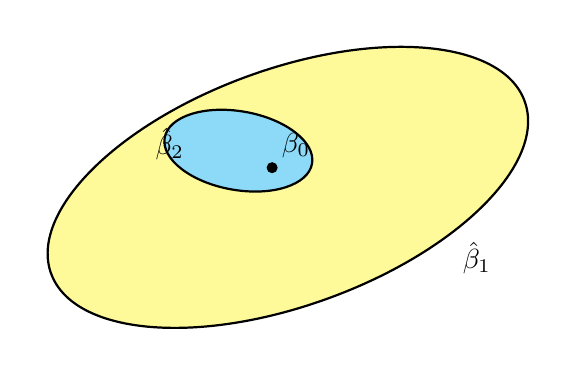
\begin{tikzpicture}
\fill[yellow!40,draw=black,thick,rotate=20] (0,0) ellipse (3.2 and 1.5);
\fill[cyan!45,draw=black,thick,rotate=-10] (-0.7,0.35) ellipse (0.95 and 0.5);
\fill (-0.2,0.25) circle (2pt) node[above right]{$\beta_0$};
\node at (-1.5,0.55) {$\hat\beta_2$};
\node at (2.4,-0.9) {$\hat\beta_1$};
\end{tikzpicture}\\
{\small $\beta_0$ مقدار واقعی است. $\hat\beta_1$ بی‌گرایش است (ناحیه زرد حول $\beta_0$ متمرکز است) ولی واریانس زیادی دارد؛ $\hat\beta_2$ کمی گرایش دارد ولی واریانسش بسیار کمتر است و در مجموع \lr{MSE} کمتری دارد.}
\end{center}

همان‌گونه که مشاهده می‌شود، گاهی بهتر است برای پایین آوردن \lr{Variance}، مقداری \lr{Bias} را تحمل کرد.

\begin{example}[تخمین واریانس: گرایش در برابر واریانس]
برای نمونه‌های \lr{i.i.d.} گاوسی، تخمین‌گرهای $\hat\sigma^2_c=c\sum_{i=1}^n(X_i-\bar X)^2$ را در نظر بگیرید. کدام $c$ کمترین \lr{MSE} را می‌دهد؟
\begin{solution}
برای گاوسی می‌توان نشان داد $\frac{1}{\sigma^2}\sum(X_i-\bar X)^2\sim\chi^2(n-1)$ با میانگین $n-1$ و واریانس $2(n-1)$. پس با $W=\sum(X_i-\bar X)^2$:
$\E[cW]=c(n-1)\sigma^2$ و $\Var(cW)=2c^2(n-1)\sigma^4$، و
\[
\mathrm{MSE}(c)=\sigma^4\big[(c(n-1)-1)^2+2c^2(n-1)\big].
\]
با مشتق‌گیری: $c^*=\frac{1}{n+1}$. مقایسه:
\begin{center}
\renewcommand{\arraystretch}{1.4}
\begin{tabular}{c|c|c|c}
$c$ & گرایش & $\mathrm{MSE}/\sigma^4$ & برای $n=10$\\\hline
$\frac{1}{n-1}$ (بی‌گرایش) & $0$ & $\frac{2}{n-1}$ & $0.222$\\
$\frac1n$ & $\frac{\sigma^2}{n}$ & $\frac{2n-1}{n^2}$ & $0.190$\\
$\frac{1}{n+1}$ & $\frac{2\sigma^2}{n+1}$ & $\frac{2}{n+1}$ & $0.182$
\end{tabular}
\end{center}
تخمین‌گر بی‌گرایش بیشترین \lr{MSE} را دارد! با پذیرش کمی گرایش، واریانس به اندازه‌ای کم می‌شود که خطای کل کمتر شود.
\end{solution}
\end{example}

\begin{example}[تخمین پارامتر یکنواخت]
برای $\mathcal U(0,\theta)$ سه تخمین‌گر $\hat\theta_1=2\bar X_n$، $\hat\theta_2=\max_iX_i$ و $\hat\theta_3=\frac{n+1}{n}\max_iX_i$ را از نظر \lr{MSE} مقایسه کنید.
\begin{solution}
\begin{itemize}
\item $\hat\theta_1$: بی‌گرایش، $\Var=4\cdot\frac{\theta^2}{12n}=\frac{\theta^2}{3n}$؛ $\mathrm{MSE}=\frac{\theta^2}{3n}$.
\item $\hat\theta_2$: با $f_U(u)=\frac{nu^{n-1}}{\theta^n}$: $\E U=\frac{n\theta}{n+1}$ و $\E U^2=\frac{n\theta^2}{n+2}$؛ پس $\Var U=\frac{n\theta^2}{(n+1)^2(n+2)}$ و $\mathrm{Bias}=\frac{\theta}{n+1}$. $\mathrm{MSE}=\frac{2\theta^2}{(n+1)(n+2)}$.
\item $\hat\theta_3$: بی‌گرایش، $\mathrm{MSE}=\Var=\frac{(n+1)^2}{n^2}\cdot\frac{n\theta^2}{(n+1)^2(n+2)}=\frac{\theta^2}{n(n+2)}$.
\end{itemize}
برای $n=10$: $0.0333\theta^2$، $0.0152\theta^2$ و $0.0083\theta^2$. تخمین‌گرهای مبتنی بر بیشینه، خطایی از مرتبه $\frac1{n^2}$ دارند (در مقابل $\frac1n$ برای میانگین) ــ تفاوتی بسیار چشمگیر برای $n$ بزرگ.
\end{solution}
\end{example}

\subsection{انواع تخمین‌گرهای نقطه‌ای}
\begin{itemize}
\item تخمین‌گر بی‌گرایش (\lr{unbiased}) و دارای کمینه واریانس:\\ \lr{(Minimum-Variance Unbiased Estimator --- \textcolor{red!70!black}{MVUE})}
\item تخمین‌گر کمینه میانگین مربعات خطا:\\ \lr{(Minimum Mean Square Estimator --- \textcolor{red!70!black}{MMSE})}
\item تخمین‌گر بیشینه درست‌نمایی:\\ \lr{(Maximum Likelihood Estimator --- \textcolor{red!70!black}{MLE})}
\item تخمین‌گر مبتنی بر گشتاور:\\ \lr{(Method of Moments Estimator --- \textcolor{red!70!black}{MoME})}
\item و بسیاری دیگر\ldots
\end{itemize}
(دو مورد آخر در جلسات بعد به تفصیل بررسی می‌شوند.)

\section{تمرین‌های تکمیلی}

\begin{exercise}
$X$ و $N$ مستقل‌اند، $X\sim\mathcal N(0,4)$ (سیگنال) و $N\sim\mathcal N(0,1)$ (نویز). مشاهده $Y=X+N$ است. بهترین تخمین \lr{MS} برای $X$ از روی $Y$ و خطای آن را بیابید.
\end{exercise}
\begin{solution}
$X,Y$ مشترکاً گاوسی‌اند (ترکیب خطی گاوسی‌های مستقل). $\Cov(X,Y)=\Var X=4$، $\Var Y=5$. پس $\hat X=\E(X\given Y)=\frac45Y$ (تخمین خطی و غیرخطی یکی است). خطا: $\sigma_X^2(1-\rho^2)=4\big(1-\frac{16}{4\cdot5}\big)=\frac45=0.8$ (در مقایسه با خطای $1$ اگر از خود $Y$ استفاده می‌کردیم، و $4$ اگر $Y$ را نادیده می‌گرفتیم).
\end{solution}

\begin{exercise}
نشان دهید $\E\big[\Var(Y\given X)\big]+\Var\big(\E(Y\given X)\big)=\Var(Y)$ (قانون واریانس کل) و تعبیر آن را در قالب تخمین \lr{MS} بیان کنید.
\end{exercise}
\begin{solution}
$\Var Y=\E Y^2-(\E Y)^2=\E[\E(Y^2\given X)]-(\E[\E(Y\given X)])^2=\E[\Var(Y\given X)+\E(Y\given X)^2]-(\E[\E(Y\given X)])^2=\E[\Var(Y\given X)]+\Var(\E(Y\given X))$.
\textbf{تعبیر:} جمله اول خطای تخمین‌گر غیرخطی بهینه $\E[(Y-\E(Y\given X))^2]$ است؛ جمله دوم واریانس «توضیح‌داده‌شده» توسط $X$. واریانس کل = خطای باقی‌مانده + بخش قابل پیش‌بینی.
\end{solution}

\begin{exercise}
برای $\mathrm{Pois}(\lambda)$، تخمین‌گر $\hat\lambda=\bar X_n$ را از نظر گرایش، واریانس، \lr{MSE} و سازگاری بررسی کنید.
\end{exercise}
\begin{solution}
$\E\hat\lambda=\lambda$ (بی‌گرایش). $\Var\hat\lambda=\frac{\lambda}{n}$. $\mathrm{MSE}=\frac\lambda n\to0$؛ پس سازگار است.
\end{solution}
